%\chapter 7
\chapter{OCT 2010}
\section{Q5 QCT 2010}
\shabox{Q5 OCT 2010}
\begin{figure}[!ht]
\centering
 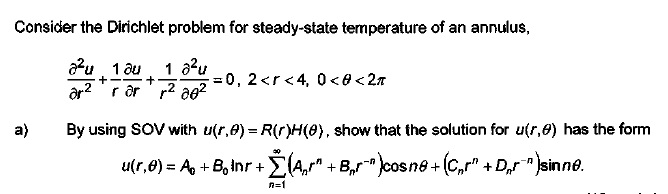
\includegraphics[width=0.8\textwidth]{q8oct10.jpg}    %insert your file at 'imagey1'
%\caption{$\mathbb{Z}_6$} \label{z6}
\end{figure}
\begin{figure}[!ht]
\centering
 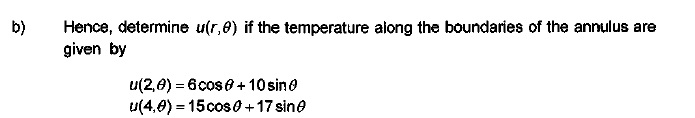
\includegraphics[width=0.8\textwidth]{q8oct10a.jpg}    %insert your file at 'imagey1'
%\caption{$\mathbb{Z}_6$} \label{z6}
\end{figure}\\
%----------------
\shabox{Solution}\\
a)
By using SOV $u(r,\theta)=R(r)H(\theta)$ and substitute into PDE gives two ODEs
\begin{align}
rR^{''}+rR^{'}-\lambda R&=0\label{q5oc10a}\\
H^{''}+\lambda H&=0\label{q5oc10b}
\end{align}
 We are seeking a solution of the \underline{$H(\theta)$-Problem }
 \begin{equation}
H^{''}+\lambda H=0,\,H(\theta)=H(\theta+2\pi)\label{q5oc11c}
\end{equation}
It will form an orthogonal set on the interval $[0,2\pi]$.\\
The three possible general solution s of \eqref{q5oc10b},
\begin{align}
H(\theta)&=c_1+c_2\theta,\,\,\lambda=0\label{q5oc11e}\\
H(\theta)&=c_1\,\cosh\,\alpha\theta+c_2\,\sinh\,\alpha\theta,\,\,\lambda=-\alpha^2<0\label{q5oc11f}\\
H(\theta)&=c_1\,\cos\,\alpha\theta+c_2\,\sin\,\alpha\theta,\,\,\,\lambda=\alpha^2>0\label{q5oc11g}
\end{align}
Solution \eqref{q5oc11e} is periodic if $C_2=0$. Similarly, solution \eqref{q5oc11f} is periodic if $c_1=c_2=0$.The constant solution
\begin{equation}
H(\theta)=c_1\label{soq5oc11a}
\end{equation}
can be assigned any period, and so $\lambda=0$ is an eigenvalue.\\
Solution \eqref{q5oc11g} will be $2\pi$-periodic if $\alpha=n$, where $n=1,2,\ldots$. \\The eigenvalues of \eqref{q5oc11g} are $\lambda_0=0$ and $\lambda_n=n^2,\,n=1,2,\ldots$.\\
The correspondence  eigenfunctions are
\begin{align}
H(\theta)&=c_1,\,n=0\label{soq5oc11a}\\
H(\theta)&=c_1\,\cos\,n\theta+c_2\,\sin\,n\theta,\,\,n=1,2,\ldots\label{soq5oc11c}
\end{align}
\underline{$R(r)$-Problem}:\\
The Chauchy-Euler DE \eqref{q5oc10a} are
\begin{align}
R(r)&=c_1+c_2\,\ln\,r,\,\,n=0\label{soq5oc11d}\\
R(r)&=c_1r^n+c_2r^{-n}\,\,n=1,2\ldots\label{soq5oc11e}
\end{align}
Thus product solution $u_n=R(r)H(\theta)$ for Laplace's equation  polar are
\begin{align*}
u_0&=(c_1+c_2\,\ln\,r)(c_1)\\
&=c_1c_1+c_1c_2\,\ln\,r\\
&=A_0+B_0\,\ln\,r\leftarrow\shabox{$A_0=c_1c_1$ and $B_0=c_1c_2$}\\
u_n&=(c_1r^n+c_2r^{-n})(c_1\,\cos\,n\theta+c_2\,\sin\,n\theta)\\
&=(c_1c_1r^n+c_1c_2r^{-n})\cos\,n\theta+(c_1c_2r^n+c_2c_2r^{-n})\sin\,n\theta\\
&=(A_nr^n+B_nr^{-n})\cos\,n\theta+(C_nr^n+D_nr^{-n})\sin\,n\theta
\end{align*}
The superposition principle then gives the solution
\begin{equation}
u(r,\theta)=A_0+B_0\,\ln\,r+\sum_{n=1}^\infty\,\left((A_nr^n+B_nr^{-n})\cos\,n\theta+(C_nr^n+D_nr^{-n})\sin\,n\theta\right)\label{soq5oc11f}
\end{equation}
b)\\
\underline{Apply BC: $u(2,\theta)=6\,cos\,\theta+ 10\,\sin\,\theta$}
\begin{align*}
u(2,\theta)=6\,\cos\,\theta+ 10\,\sin\,\theta&=A_0+B_0\ln\,2+\sum_{n=1}^\infty\,\left((A_n2^n+B_n2^{-n})\cos\,n\theta+(C_n2^n+D_n2^{-n})\sin\,n\theta\right)\\
%----------------
A_0+B_0\,\ln\,2&=\frac{1}{2\pi}\int_0^{2\pi}(6\,\cos\,\theta+ 10\,\sin\,\theta)d\theta\\
&=\frac{1}{2\pi}\left[6\,\sin\,\theta-10\,\cos\,\theta\right]_0^{2\pi}\\
&=\frac{1}{2\pi}(0-10(1-1))=0\\
%\text{So}\,\,\,\,A_0+B_0\,\ln\,r&=0
\end{align*}
%-------------------------
So
\begin{equation}
A_0+B_0\ln\,2=0\label{sor1}
\end{equation}
\begin{align}
u(2,\theta)=6\,\cos\,\theta+ 10\,\sin\,\theta&=\sum_{n=1}^\infty\,(A_n2^n+B_n2^{-n})\cos\,n\theta\\
A_n2^n+B_n2^{-n}&=\frac{1}{\pi}\int_0^{2\pi}(6\,\cos\,\theta+10\,\sin\,\theta)\cos\,n\theta\\
&=\frac{1}{\pi}\left(\int_0^{2\pi}\,6\,cos\,\theta\,\cos\,n\theta\,d\theta+\int_0^{2\pi}10\,\sin\,\theta\,\cos\,n\theta\right)\\
\text{when}\,\,n=1&\\
2A_1+\frac{B1}{2}&=\frac{1}{\pi}(6\pi)+0\\
&=6
\end{align}
Thus 
\begin{equation}
4A_1+B_1=12\label{sor2}
\end{equation}
\begin{align*}
C_n2^n+D_n2^{-n}&=\frac{1}{\pi}\int_0^{2\pi}[6\,\cos\,\theta+10\,\sin\,\theta]\sin\,n\theta\,d\theta\\
%\text{When $n$=1}&\\
2C_1+\frac{D_1}{2}&=\frac{1}{\pi}\int_0^{2\pi}6\,\cos\,\theta\,\sin\,\theta\,d\theta+\frac{1}{\pi}\int_0^{2\pi}\,10\,\sin\,\theta\,\sin\,\theta\,d\theta\\
&=\frac{1}{\pi}\sin^2\,\theta\big|_0^{2\pi}+\frac{10}{\pi}\int_0^{2\pi}\sin^2\,\theta\,d\theta\\
&=0+\frac{10}{\pi}\int_0^{2\pi}\frac{1-\cos\,2\theta}{2}\\
&=\frac{10}{\pi}\left[\frac{\theta}{2}-\frac{1}{4}\sin\,2\theta\right]_0^{2\pi}\\
&=10\\
\text{So}\,\,2C_1+\frac{D_1}{2}&=10
\end{align*}
Thus
\begin{equation}
4C_1+D_1=20\label{sorr1}
\end{equation}
\underline{Now apply BC: $u(4,\theta)=15\,\cos\,\theta+17\,\sin\,\theta$}:
\begin{align*}
A_0+B_0\, \ln\,4&=\frac{1}{2\pi}\int_0^{2\pi}(15\,\cos\,\theta+17\,\sin\,\theta)d\theta\\
&=0
\end{align*}
Thus
\begin{align}
A_0+B_0\ln\,4&=0\label{ssr1}
\end{align}
From \eqref{so1} and \eqref{ssr1} give $A_0=0,\,B_0=0$.\\
Next,
\begin{align*}
A_n4^n+B_n4^{-n}&=\frac{1}{\pi}\int_0^{2\pi}(15\,\cos\,\theta+17\,\sin\,\theta)\cos\,n\theta\,d\theta\\
4A_1+\frac{B_1}{4}&=\frac{1}{\pi}\int_0^{2\pi}(15\,\cos\,\theta\,\cos\,\theta+17\,\sin\,\theta\,\cos\,\theta)d\theta\leftarrow\shabox{Orthogonal series expansion: $n=1$}\\
&=\frac{1}{\pi}(15\pi+0)\\
&=15\\
\text{so},\,\,4A_1+\frac{B_1}{4}&=15
\end{align*}
Thus 
\begin{equation}
16A_1+B_1=60\label{ssr2}
\end{equation}
From \eqref{sor2} and \eqref{ssr2}; \eqref{ssr2}-\eqref{sor2} gives
\begin{align*}
12A_1&=48\\
A_1&=4\\
16(4)+B_1&=60\\
B_1&=-4
\end{align*}
Finally, 
\begin{align*}
C_n4^n+D_n4^{-n}&=\frac{1}{\pi}\int_0^{2\pi}(15\,\cos\,\theta+17\,\sin\,\theta)\sin\,n\theta\,d\theta\\
4C_1+\frac{D_1}{4}&=\frac{1}{\pi}\int_0^{2\pi}(15\,\cos\,\theta\,\sin\,\theta+17\,\sin\,\theta\,\sin\,\theta)d\theta\leftarrow\shabox{Orthogonal series expansion: $n=1$}\\
&=\frac{1}{\pi}(0+17\pi)\\
&=17\\
\text{so},\,\,4A_1+\frac{B_1}{4}&=17
\end{align*}
Thus 
\begin{equation}
16C_1+D_1=68\label{sorr2}
\end{equation}
Apply \eqref{sorr1} and \eqref{sorr2}, we solve for $C_1$ and $D_1$. \eqref{sorr2}-\eqref{sorr1} gives
\begin{align*}
12C_1&=48\\
C_1&=4\\
16(4)+D_1&=68\\
D_1&=4
\end{align*}
The solution is
\begin{equation}
u(r,\theta)=(4r-4r^{-1})\cos\,\theta+(4r+4r^{-1})\sin\,\theta
\end{equation}
\subsection{Q4 APR 2010}
\shabox{Q4}
\begin{figure}[!ht]
\centering
 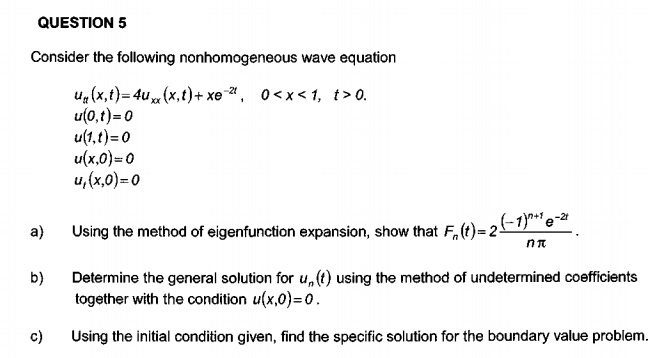
\includegraphics[width=\textwidth]{q5ap10.jpg}    %insert your file at 'imagey1'
%\caption{$\mathbb{Z}_6$} \label{z6}
\end{figure}\\
\shabox{Solution}\\
a)\\
The eigenvalues and eigenfunctions of 
\begin{equation}
%\end{}
X^{''}+\lambda X=0, X(0)=0,\,X(1)=0
\end{equation}
are found to be 
\begin{equation}
\lambda_n=\alpha_n^2=n^2\pi^2\,\,\text{and}\,\,\sin\,n\pi x,\,n=1,2,3,\ldots
\end{equation}
If we assume that
\begin{align}
u(x,t)&=\sum_{n=1}^\infty\,u_n(t)\,\sin\,n\pi x\nonumber\\
u_{xx}&=\sum_{n=1}^\infty\,u_n(t)(-n^2\pi^2)\,\sin\,n\pi x\label{q4ap10a}\\
u_{tt}&=\sum_{n=1}^\infty\,u_n^{''}(t)\,\sin\,n\pi x\label{q4ap10b}
\end{align}
We can write $F(x,t)=xe^{-2t}$
\begin{align}
xe^{-2t}&=\sum_{n=1}^\infty\,F_n(t)\,\sin\,n\pi x\nonumber\\
F_n(t)&=\frac{2}{1}\int_0^1\,xe^{-2t}\sin\,n\pi x\,dx\\
&=2e^{-2t}\int_0^1\,x\,\sin\,n\pi x\,dx\nonumber\\
&=2e^{-2t}\left[\frac{-x}{n\pi}\cos\,n\pi x+\frac{1}{n\pi}\int\,\cos\,n\pi x\,dx\right]\nonumber\\
&=2e^{-2t}\left[-\frac{x}{n\pi}\,\cos\,n\pi x+\frac{1}{n^2\pi^2}\sin\,n\pi x\right]_0^1\\
&=2e^{-2t}\left(\frac{-1}{n\pi}(-1)^n\right)\nonumber\\
&=2e^{-2t}\left(\frac{1}{n\pi}(-1)^{n+1}\right)\nonumber\\
xe^{-2t}&=\sum_{n=1}^\infty\left(2e^{-2t}\left(\frac{1}{n\pi}(-1)^{n+1}\right)\right)\sin\,n\pi x\label{q4ap10c}
\end{align}
%------------------
So $F_n(t)=2\left(\frac{(-1)^{n+1}}{n\pi}\right)e^{-2t}$


b) Substitute \eqref{q4ap10a}, \eqref{q4ap10b} and \eqref{q4ap10c} into PDE gives
\begin{align}
u_{tt}-4u_{xx}&=xe^{-2t}\\
\sum_{n=1}^\infty\,\left[u_n^{''}(t)+4n^2\pi^2u_n(t)\right]\sin\,n\pi x&=\sum_{n=1}^\infty\left(2e^{-2t}\left(\frac{1}{n\pi}(-1)^{n+1}\right)\right)\sin\,n\pi x\label{q4ap10d}
\end{align}
By equating the coefficients of $\sin\,n\pi x$,
\begin{align}
u_n^{''}(t)+4n^2\pi^2u_n(t)&=2e^{-2t}\left(\frac{1}{n\pi}(-1)^{n+1}\right)\label{q4ap10e}
%u_n^{''}&=\frac{(-1)^{n+1}}{n\pi}2e^{-2t}-4n^2\pi^2u_n(t)\\
%u_n^{'}&=
\end{align}
Solve \eqref{q4ap10e} by using undetermined coefficients;
Auxiliary equation
\begin{align*}
m^2+4n^2\pi^2&=0\\
m&=2n\pi i,\,-2n\pi i\leftarrow\shabox{complex roots}
\end{align*}
The complementary solution,
\begin{equation}
u_{nc}(t)=c_1\,\cos\,2n\pi t+c_2\,\sin\,2n\pi t\label{a4ap10f}
\end{equation}
Particular solution 
\begin{align*}
u_{np}(t)&=Be^{-2t}\\
u^{'}&=-2Be^{-2t}\\
u^{''}&=4Be^{-2t}\\
%&=4(Bx+c)e^{-2t}-4Be^{-2t}
\end{align*}
Substitute into \eqref{q4ap10e} gives
\begin{align*}
4Be^{-2t}+4n^2\pi^2Be^{-2t}&=\left(\frac{2(-1)^{n+1}}{n\pi}\right)\\
%(4C-4B+4n^2\pi^2C)e^{-2t}+(4B+4n^2\pi^2)xe^{-2t}&=\left(\frac{(-1)^{n+1}}{n\pi}\right)2e^{-2t}\\
\end{align*}
By equating the coefficient of  and $e^{-2t}$ becomes
\begin{align}
B(4+4n^2\pi^2)&=\left(\frac{2(-1)^{n+1}}{n\pi}\right)
%B+2n^2\pi^2&=\left(\frac{(-1)^{n+1}}{n\pi}\right)\label{sso1}\\
\label{sso2}
\end{align}
From \eqref{sso2} gives
\begin{equation}
B=\frac{(-1)^{n+1}}{2n\pi(1+n^2\pi^2)}\label{sso3} 
\end{equation}

%subtitute \eqref{sso3} into \eqref{sso1}
%\begin{align*}
%4C+4n^2\pi^2+2n^2\pi^2&=\left(\frac{(-1)^{n+1}}{n\pi}\right)\\
%4C&=\left(\frac{(-1)^{n+1}}{6n^3\pi^3}\right)\\
%C&=\left(\frac{(-1)^{n+1}}{24n^3\pi^3}\right)\\
%u_p(t)&=
%\end{align*}
Thus the particular solution
\begin{equation}
u_{np}(t)=\left(\frac{(-1)^{n+1}}{2n\pi(1+n^2\pi^2)}\right)e^{-2t}
\end{equation}
Hence the general solution
\begin{align*}
u_n(t)&=u_{nc}+u_{np}\\
&=c_1\,\cos\,2n\pi t+c_2\,\sin\,2n\pi t+\left(\frac{(-1)^{n+1}}{2n\pi(1+n^2\pi^2)}\right)e^{-2t}
\end{align*}
Apply $u(x,0)=0$:
\begin{align*}
u_n(x,0)=0&=c_1(1)+0+\frac{(-1)^{n+1}}{2n\pi(1+n^2\pi^2)}\\
c_1&=\frac{(-1)^{n+2}}{2n\pi(1+n^2\pi^2)}
\end{align*}
Hence the general solution
\begin{align}
u_n(t)&=\left(\frac{(-1)^{n+2}}{2n\pi(1+n^2\pi^2)}\right)\cos\,2n\pi t+c_2\,\sin\,2n\pi t+\left(\frac{(-1)^{n+1}}{2n\pi(1+n^2\pi^2)}\right)e^{-2t}
\end{align}
%--------------------
c) 
The solution,

\begin{align}
u(x,t)&=\sum_{n=1}^\infty\left[\left(\frac{(-1)^{n+2}}{2n\pi(1+n^2\pi^2)}\right)\cos\,2n\pi t+c_2\,\sin\,2n\pi t+\left(\frac{(-1)^{n+1}}{2n\pi(1+n^2\pi^2)}\right)e^{-2t}\right]\sin\,n\pi x\label{sss1}
\end{align}
Apply BC: $u_t(x,0)=0$:
\begin{align}
u_t(x,t)&=\sum_{n=1}^\infty\left[\left(2\frac{(-1)^{n+2}}{2n\pi(1+n^2\pi^2)}\right)(-\sin\,2n\pi t)+2c_2\,\cos\,2n\pi t-2\left(\frac{(-1)^{n+1}}{2n\pi(1+n^2\pi^2)}\right)e^{-2t}\right]\sin\,n\pi x\nonumber\\
0&=2c_2-2\left(\frac{(-1)^{n+1}}{2n\pi(1+n^2\pi^2)}\right)\nonumber\\
c_2&=\left(\frac{(-1)^{n+1}}{2n\pi(1+n^2\pi^2)}\right)\label{ssss1}
\end{align}
Hence the solution VBP is given by \eqref{sss1} where $c_2$ is given by \eqref{ssss1}.

